%
% $RCSfile: schema.tex,v $
%
% Copyright (C) 2002-2008. Christian Heller.
%
% Permission is granted to copy, distribute and/or modify this document
% under the terms of the GNU Free Documentation License, Version 1.1 or
% any later version published by the Free Software Foundation; with no
% Invariant Sections, with no Front-Cover Texts and with no Back-Cover
% Texts. A copy of the license is included in the section entitled
% "GNU Free Documentation License".
%
% http://www.cybop.net
% - Cybernetics Oriented Programming -
%
% http://www.resmedicinae.org
% - Information in Medicine -
%
% Version: $Revision: 1.1 $ $Date: 2008-08-19 20:41:08 $ $Author: christian $
% Authors: Christian Heller <christian.heller@tuxtax.de>
%

\subsection{Schema}
\label{schema_heading}
\index{Schema with Meta Information}
\index{Knowledge Schema with Meta Information}
\index{Model}
\index{Concept}
\index{Item}
\index{Category}
\index{Compound}
\index{Discrimination}
\index{Categorisation}
\index{Composition}
\index{Compound Model}
\index{Meta Information}
\index{Meta Model}

A theoretical \emph{Model} is an abstract clip of the real world, and exists in
the human mind. Another common word for \emph{Model} is \emph{Concept}. It is
the subsumption of \emph{Item}, \emph{Category} and \emph{Compound}, resulting
from three activities of abstraction: \emph{Discrimination}, \emph{Categorisation}
and \emph{Composition} (section \ref{abstraction_heading}). As such, each model
\emph{knows} about the parts it consists of.

\begin{figure}[ht]
    \begin{center}
        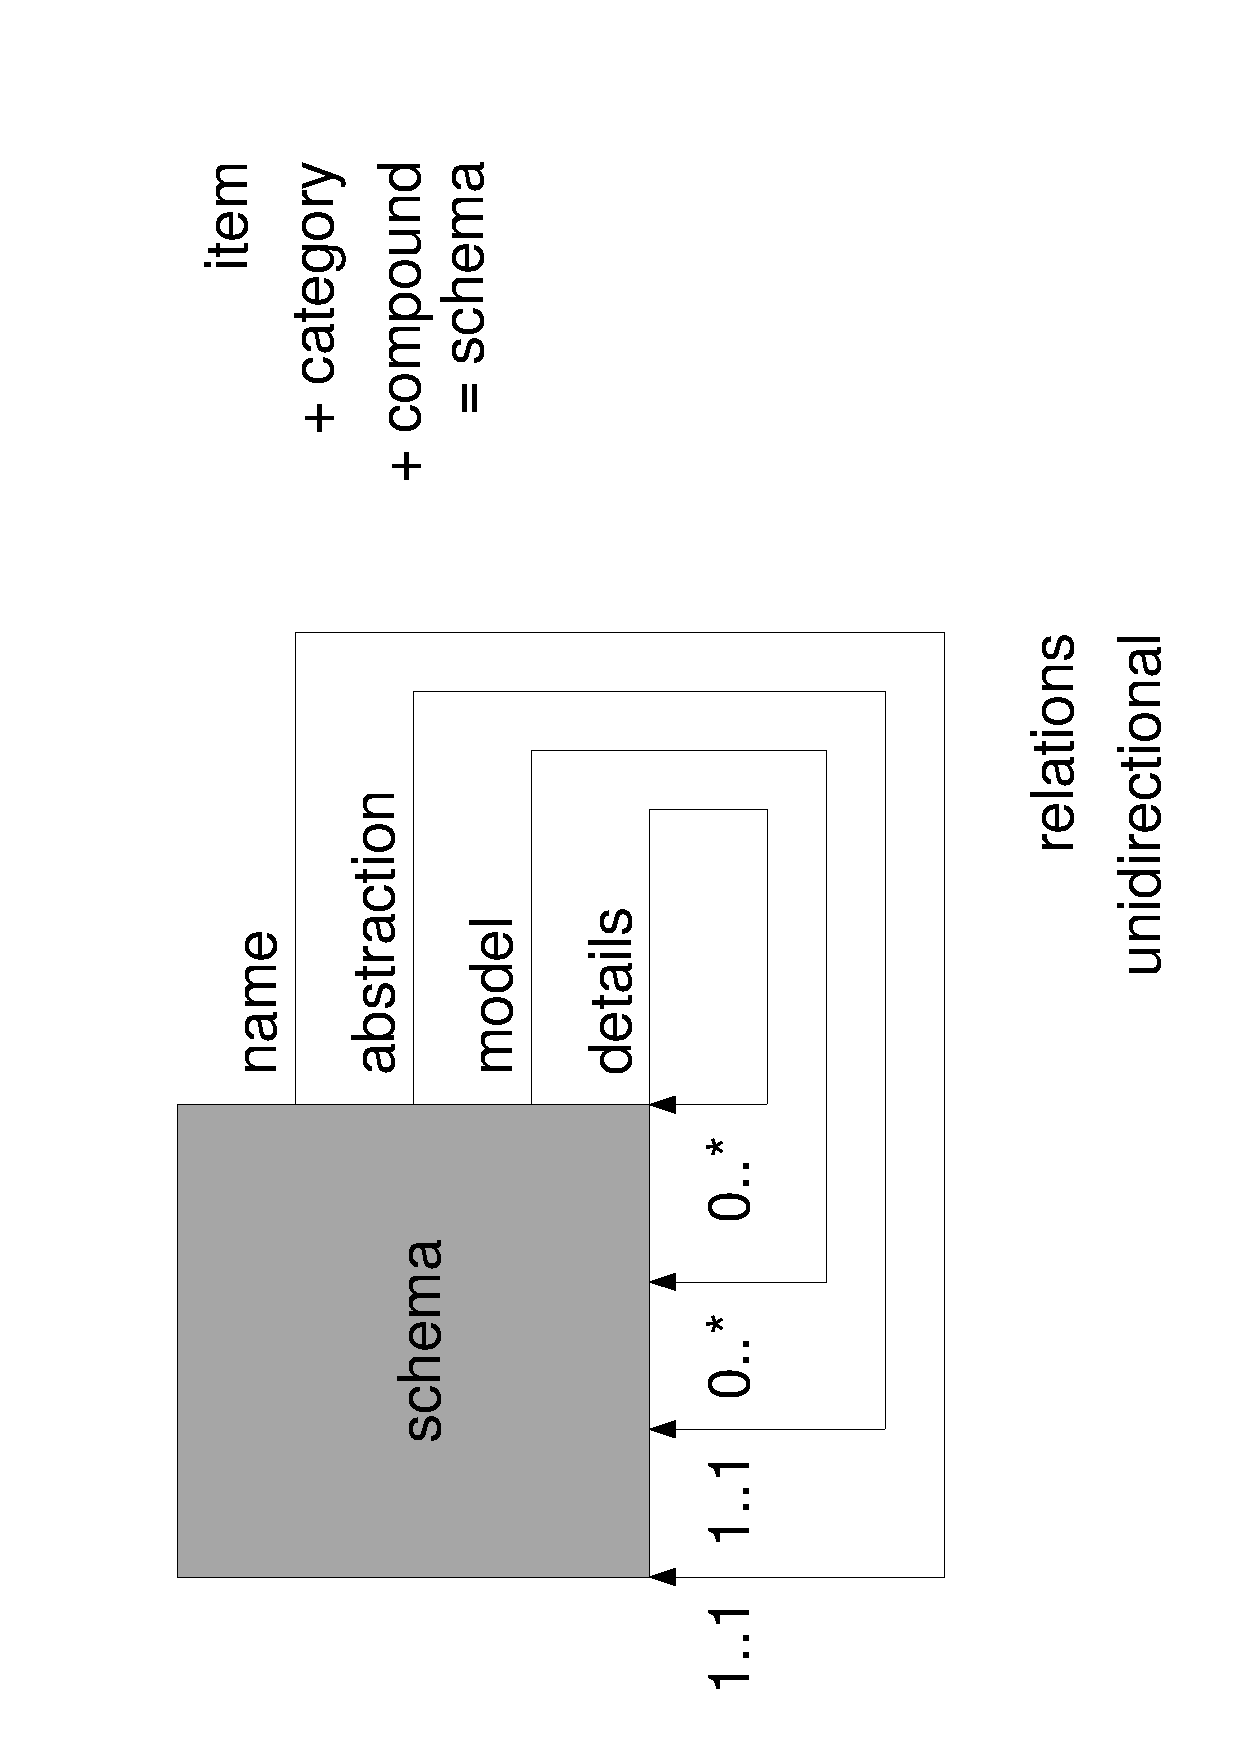
\includegraphics[scale=0.3,angle=-90]{graphic/schema.pdf}
        \caption{Knowledge Schema with Meta Information about Parts}
        \label{schema_figure}
    \end{center}
\end{figure}

Yet what does this knowledge of a compound model (whole) about its parts imply?
Software developers call knowledge \emph{about} something \emph{Meta Information}.
Figure \ref{schema_figure} shows the four essential kinds of meta information in
a whole-part relation. Software developers might want to call the illustration
of these relations a \emph{Schema} or \emph{Meta Model}.

An obvious way is to give each part a unique \emph{Name} for identification.
The concept of a human body, for example, would have parts like heart, brain,
left\_arm and so on.

Secondly, a compound needs to know about the \emph{Model} of each part since a
part may itself be seen as compound that needs to know about its parts. Although
all real world items can be modelled as compound, it does not make sense to do
so in the virtual world of the human mind. As mentioned before, models have to
be limited in their information contents, towards microcosm as well as towards
macrocosm, in order to be comprehensible by the human mind. It is therefore
necessary to introduce primitive models like a word or a number (compare
\emph{Quality and Quantity}, section \ref{quality_and_quantity_heading}),
representing the final form of abstraction in a compound.

The distinction of the several kinds of models, in other words the kind of
\emph{Abstraction} (compound, term, number etc.) of a model is the third
kind of information a compound needs to know about its parts. It is comparable
to a \emph{Type} in classical system programming languages (section
\ref{system_programming_heading}).

All further kinds of meta information are summed up by a fourth relation which
is called \emph{Details} in this work. Just like the \emph{Model}, it is a
dynamically extensible structure. It will be explained in the following section.

The suggested knowledge model uses a simple \emph{Tree} structure, capable of
referencing parts of arbitrary type. It does not follow the \emph{Composite}
software pattern (section \ref{composite_heading}), because the meta information
whether a part model is a compound (composite) or not (leaf) does not belong
into the model structure. Section \ref{categorisation_versus_composition_heading}
explained this design mistake on the example of \emph{Party} types. It is not
good to fix some model as leave, at design time. Who knows if at runtime
(during program execution), that model would not have to have any parts?
As an aside: A similar design (simple tree structure) is used by the
\emph{Java Swing} framework \cite{java}, for example. Its tree node class
\emph{DefaultMutableTreeNode} represents a \emph{Tree Node} and
\emph{Tree Container}, at the same time.
